\documentclass[aspectratio=169, 10pt, xcolor={table,dvipsnames}]{beamer}

% --- Theme & Color ---
\usetheme{Madrid}
\usecolortheme{beaver} 
\newcommand{\tool}{{\textsc{Bolt}}\xspace}
% --- Packages ---
\usepackage{booktabs}
\usepackage{multirow}
\usepackage{tikz}
\usetikzlibrary{
    shapes, arrows.meta, positioning, decorations.pathreplacing, calc,
    shadows, shapes.multipart, patterns, fit, backgrounds, graphs, trees, matrix, chains
}
\usepackage{caption}
\usepackage{lmodern} 
\usepackage{colortbl}
\usepackage{amsmath}
\usepackage{pifont} 

% --- Font Configuration ---
\renewcommand{\familydefault}{\sfdefault}

% --- Colors (Explicit RGB) ---
\definecolor{efblue}{RGB}{45,52,54}
\definecolor{efred}{RGB}{192,57,43}
\definecolor{efgreen}{RGB}{39,174,96}
\definecolor{fixedblue}{RGB}{227,242,253}
\definecolor{offsetorange}{RGB}{255,243,224}
\definecolor{heapgreen}{RGB}{232,245,233}
\definecolor{garbagegrey}{RGB}{245,245,245}
\definecolor{alertred}{RGB}{211,47,47}
\definecolor{codebg}{RGB}{250,250,250}

% --- TikZ Styles ---

% --- TikZ Styles ---
\tikzset{
    basicblock/.style={
        rectangle,
        draw=black!60,
        thick,
        fill=white,
        rounded corners=2pt,
        align=center,
        font=\footnotesize\sffamily,
        drop shadow={opacity=0.15},
        minimum height=0.9cm,
        text width=3.5cm, 
        inner sep=5pt
    },
    moduleblock/.style={
        rectangle,
        draw=black!60,
        thick,
        fill=white,
        rounded corners=4pt,
        align=center,
        font=\bfseries\small,
        drop shadow={opacity=0.15},
        minimum height=1.2cm,
        minimum width=2.2cm,
        inner sep=5pt
    },
    narrowblock/.style={
        basicblock,
        text width=2.5cm
    },
    codeblock/.style={
        rectangle,
        draw=gray!40,
        fill=codebg,
        font=\ttfamily\scriptsize,
        align=left,
        inner sep=8pt,
        rounded corners=2pt,
        drop shadow={opacity=0.05}
    },
    vecbox/.style={
        rectangle,
        draw=black!50,
        minimum width=1.1cm,
        minimum height=0.6cm,
        align=center,
        font=\scriptsize\ttfamily,
        anchor=center,
        inner sep=0pt
    },
    flow/.style={
        ->, 
        >=Stealth, 
        thick, 
        color=efblue,
        rounded corners
    },
    bitbox/.style={
        rectangle,
        draw=black!40,
        minimum width=0.8cm,
        minimum height=0.8cm,
        align=center,
        font=\bfseries\small,
        inner sep=0pt,
        fill=white,
        anchor=center
    }
}


% --- Custom Commands ---
\newcommand{\cmark}{\ding{51}}
\newcommand{\xmark}{\ding{55}}

% --- Metadata ---
\title[\tool]{\textbf{\Huge \tool}}
\subtitle{Breaking Blockchain Consensus via Boundary-Seeking Fuzzing \\ of Inter-Client State Serialization}
\author[UCSB]{Hanzhi Liu \and Yanju Chen \and Yu Feng}
\institute[UCSB]{University of California, Santa Barbara}
\date{\today}

\begin{document}

% =================================================================
% 1. INTRO
% =================================================================
\begin{frame}
    \titlepage
\end{frame}

\begin{frame}{Agenda}
    \tableofcontents
\end{frame}

% =================================================================
% 2. PROBLEM
% =================================================================
\section{Problem Definition}

\begin{frame}{The Consensus Risk: Chain Splits}
    \textbf{The Problem:} Ethereum requires exact byte-consistency (Canonicalization). 
    A logically ``Valid'' object with ``Invalid'' encoding (e.g., dirty padding) splits the chain.
    
    \vspace{0.5cm}
    \centering
    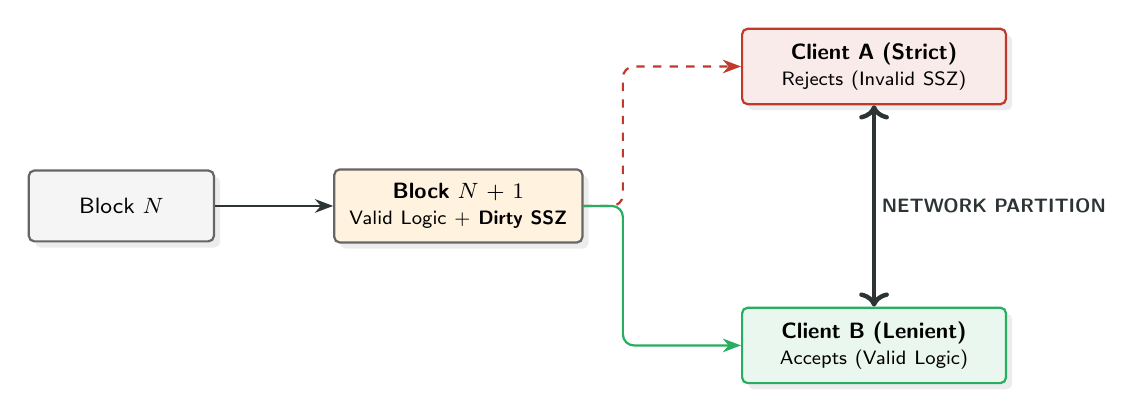
\begin{tikzpicture}[node distance=1.5cm and 1.5cm, auto]
        % Ancestor
        \node[basicblock, fill=garbagegrey, text width=2cm] (b0) {Block $N$};
        
        % The Malicious Block
        \node[basicblock, fill=offsetorange, right=of b0, text width=2.8cm] (b1) {
            \textbf{Block $N+1$}\\
            \scriptsize Valid Logic + \textbf{Dirty SSZ}
        };
        
        % Forks - Using relative positioning for symmetry
        \node[basicblock, fill=efred!10, above right=0.8cm and 2cm of b1, draw=efred, text width=3cm] (b2a) {
            \textbf{Client A (Strict)}\\
            \scriptsize Rejects (Invalid SSZ)
        };
        
        \node[basicblock, fill=efgreen!10, below right=0.8cm and 2cm of b1, draw=efgreen, text width=3cm] (b2b) {
            \textbf{Client B (Lenient)}\\
            \scriptsize Accepts (Valid Logic)
        };

        % Arrows
        \draw[flow] (b0) -- (b1);
        \draw[flow, dashed, color=efred] (b1.east) -- ++(0.5,0) |- (b2a.west);
        \draw[flow, color=efgreen] (b1.east) -- ++(0.5,0) |- (b2b.west);
        
        % Network Partition Indicator
        \draw[<->, ultra thick, efblue] (b2a.south) -- (b2b.north) 
            node[midway, fill=white, text=efblue, font=\bfseries\scriptsize, align=center, inner sep=2pt] {NETWORK PARTITION};
    \end{tikzpicture}
\end{frame}

\begin{frame}{Why Traditional Fuzzers Fail: The Coverage Blindness}
    \textbf{Root Cause:} Fuzzers optimize for Control Flow Coverage. Lenient clients often mask out dirty bits, resulting in identical execution paths for both canonical and dirty inputs.
    
    \vspace{0.5cm}
    \begin{columns}[c]
        \column{0.45\textwidth}
            \centering
            \textbf{Program Logic}
            \vspace{0.2cm}
            
            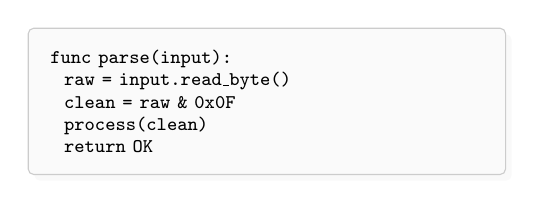
\begin{tikzpicture}
            \node[codeblock, text width=5.5cm] (code) {
                \textbf{func} parse(input):\\
                \ \ raw = input.read\_byte()\\
                % \ \ \textit{// Masking hides the dirty bit}\\
                \ \ \textbf{clean = raw \& 0x0F}\\
                \ \ process(clean)\\
                \ \ \textbf{return} OK
            };
            \end{tikzpicture}

        \column{0.55\textwidth}
            \centering
            \textbf{The Feedback Gap}
            \vspace{0.2cm}
            
            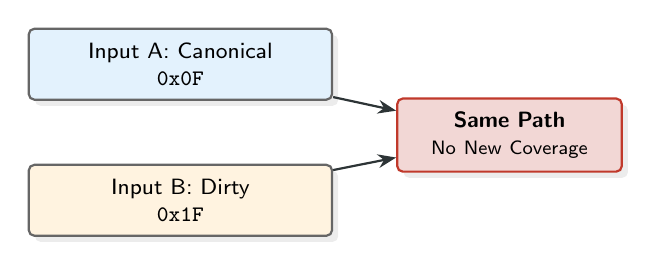
\begin{tikzpicture}[node distance=0.8cm]
                % Trace A
                \node[basicblock, fill=fixedblue, text width=3.5cm] (traceA) {Input A: Canonical\\ \texttt{0x0F}};
                
                % Trace B
                \node[basicblock, below=of traceA, fill=offsetorange, text width=3.5cm] (traceB) {Input B: Dirty\\ \texttt{0x1F}};
                
                % Comparison
                \node[basicblock, right=0.8cm of traceA, fill=efred!20, draw=efred, yshift=-0.9cm, text width=2.5cm] (result) {\textbf{Same Path}\\ \scriptsize No New Coverage};
                
                \draw[flow] (traceA) -- (result);
                \draw[flow] (traceB) -- (result);
            \end{tikzpicture}
    \end{columns}
\end{frame}

% =================================================================
% 3. SGIA DETAILED
% =================================================================
\section{Solution: SGIA}

\begin{frame}{Solution: Specification-Guided Input Abstraction (SGIA)}
    \textbf{Goal:} Transform the infinite byte space into a structured action space.
    
    \vspace{0.2cm}
    \textbf{Method:} We utilize the SSZ Schema to partition the input domain into \textbf{Semantic Buckets} via a two-stage process.
    
    \vspace{0.5cm}
    \centering
    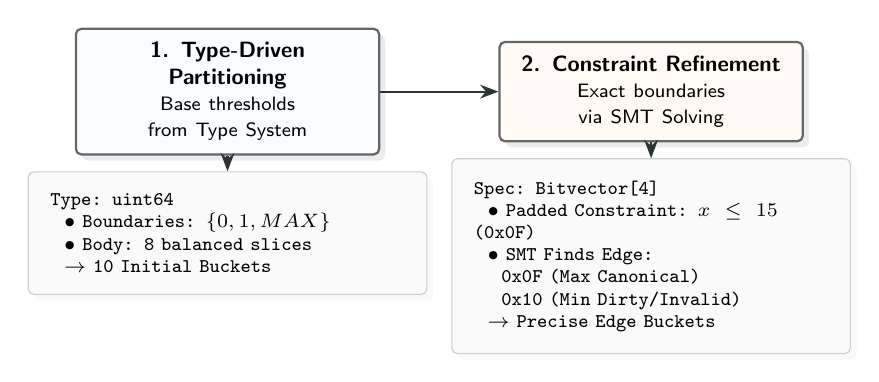
\begin{tikzpicture}[node distance=1.0cm, auto]
        % Stage 1
        \node[basicblock, fill=fixedblue!20] (stage1) {
            \textbf{1. Type-Driven Partitioning}\\
            \scriptsize Base thresholds from Type System
        };
        
        % Details 1
        \node[codeblock, below=0.2cm of stage1, text width=4.5cm] (det1) {
            \textbf{Type: \texttt{uint64}}\\
            \ \ $\bullet$ Boundaries: $\{0, 1, MAX\}$\\
            \ \ $\bullet$ Body: 8 balanced slices\\
            \ \ $\to$ \textbf{10 Initial Buckets}
        };

        % Stage 2
        \node[basicblock, right=1.5cm of stage1, fill=offsetorange!40] (stage2) {
            \textbf{2. Constraint Refinement}\\
            \scriptsize Exact boundaries via SMT Solving
        };
        
        % Details 2
        \node[codeblock, below=0.2cm of stage2, text width=4.5cm] (det2) {
            \textbf{Spec: \texttt{Bitvector[4]}}\\
            \ \ $\bullet$ Padded Constraint: $x \le 15$ (\texttt{0x0F})\\
            \ \ $\bullet$ SMT Finds Edge:\\
            \ \ \ \ \textbf{0x0F} (Max Canonical)\\
            \ \ \ \ \textbf{0x10} (Min Dirty/Invalid)\\
            \ \ $\to$ \textbf{Precise Edge Buckets}
        };
        
        % Flow
        \draw[flow] (stage1) -- (stage2);
        \draw[flow, dashed] (stage1.south) -- (det1.north);
        \draw[flow, dashed] (stage2.south) -- (det2.north);
        
    \end{tikzpicture}
\end{frame}

\begin{frame}{SGIA in Action: Concrete Bucket Catalog}
    Before fuzzing, we pre-calculate these buckets for every type. 
    The table below shows the full catalog for \texttt{Boolean} and \texttt{Bitvector[4]}.
    
    \vspace{0.2cm}
    \centering
    \begin{table}
    \scriptsize
    \renewcommand{\arraystretch}{1.2}
    \setlength{\tabcolsep}{8pt}
    \rowcolors{2}{white}{codebg} 
    \begin{tabular}{l l l l}
        \toprule
        \textbf{SSZ Type} & \textbf{Bucket} & \textbf{Value Range (Hex)} & \textbf{Semantic Intent} \\
        \midrule
        % --- Boolean Section (3 rows) ---
          & $B_{0}$ & \texttt{0x00} & Canonical False \\
          & $B_{1}$ & \texttt{0x01} & Canonical True \\
        \multirow{-3}{*}{\textbf{Boolean}} & \cellcolor{efred!20}$B_{dirty}$ & \texttt{0x02 .. 0xFF} & \textbf{Invalid / Dirty} (Non-canonical) \\
        \hline
        % --- Bitvector Section (6 rows) ---
          & $B_{0}$ & \texttt{0x00 .. 0x15} & Low Values \\
          & $B_{1}$ & \texttt{0x16 .. 0x2B} & ... \\
          & $B_{5}$ & \texttt{0x6E .. 0x83} & Mid Range \\
          & ... & ... & ... \\
          & $B_{10}$ & \texttt{0xDC .. 0xF1} & High Values \\
        \multirow{-6}{*}{\textbf{Bitvector[4]}} & \cellcolor{efred!20}$B_{11}$ & \texttt{0xF2 .. 0xFF} & \textbf{Dirty Padding} (Sets high bits) \\
        \bottomrule
    \end{tabular}
    \end{table}
    
    \vspace{0.1cm}
    \raggedright
    \scriptsize
    \textbf{Note:} For a \texttt{Bitvector[4]} (1 byte), only the lowest 4 bits are valid (max \texttt{0x0F}). Sampling from $B_{11}$ (\texttt{>0xF2}) guarantees that the upper padding bits are set, forcing a dirty encoding.
\end{frame}

\begin{frame}{The Fuzzing Logic: Probing the Schema}
    \textbf{Core Logic:} Given a target schema, the RL Agent constructs an input by selecting one bucket for each field.
    
    \vspace{0.6cm}
    \centering
    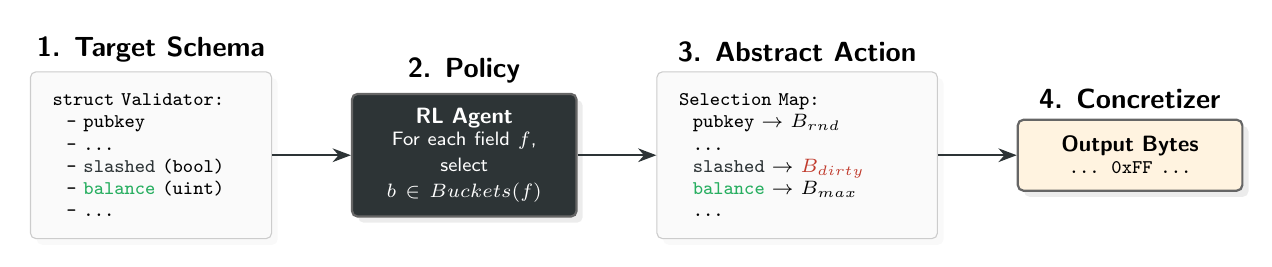
\begin{tikzpicture}[node distance=0.5cm, auto]
        % Schema
        \node[codeblock, text width=2.5cm, label=above:\textbf{1. Target Schema}] (schema) {
            \textbf{struct Validator}:\\
            \ \ - pubkey\\
            \ \ - \dots\\
            \ \ - \textcolor{efblue}{slashed} (bool)\\
            \ \ - \textcolor{efgreen}{balance} (uint)\\
            \ \ - \dots
        };
        
        % RL Agent
        \node[basicblock, right=1.0cm of schema, fill=efblue, text=white, text width=2.5cm, label=above:\textbf{2. Policy}] (rl) {
            \textbf{RL Agent}\\
            \scriptsize For each field $f$,\\
            select $b \in Buckets(f)$
        };
        
        % Action Map
        \node[codeblock, right=1.0cm of rl, text width=3.0cm, label=above:\textbf{3. Abstract Action}] (action) {
            \textbf{Selection Map:}\\
            \ \ pubkey $\to$ $B_{rnd}$\\
            \ \ \dots\\
            \ \ \textcolor{efblue}{slashed} $\to$ \textcolor{efred}{$B_{dirty}$}\\
            \ \ \textcolor{efgreen}{balance} $\to$ $B_{max}$\\
            \ \ \dots
        };

        % Concretizer
        \node[basicblock, right=1.0cm of action, fill=offsetorange, text width=2.5cm, label=above:\textbf{4. Concretizer}] (conc) {
            \textbf{Output Bytes}\\
            \scriptsize \texttt{... 0xFF ...}\\
            % \tiny (Probing Dirty Boolean \& Max Int)
        };
        
        \draw[flow] (schema) -- (rl);
        \draw[flow] (rl) -- (action);
        \draw[flow] (action) -- (conc);
        
    \end{tikzpicture}
\end{frame}

% =================================================================
% 4. REWARD MECHANISM
% =================================================================
\section{Reward Mechanism}

\begin{frame}{Execution Trace Modeling: Features in High-Dim Space}
    \textbf{Definition:} Trace = Vector of \textbf{Observed Values} for every variable.
    
    \vspace{0.2cm}
    \textbf{Key Insight:} Different branches use \textbf{independent IDs} for the same variable. Unvisited paths yield \texttt{Nil}.
    
    \vspace{0.4cm}
    \begin{columns}[T]
        \column{0.45\textwidth}
            \centering
            \textbf{1. Variable Observation Logic}
            \vspace{0.2cm}
            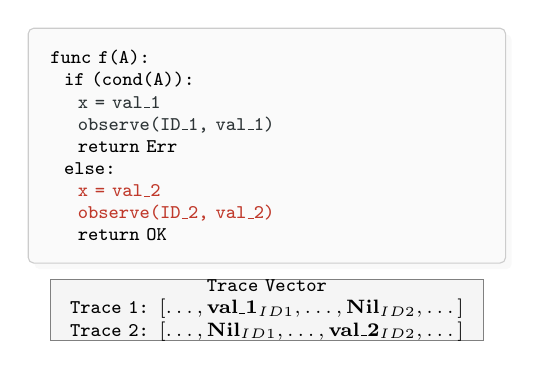
\begin{tikzpicture}
                \node[codeblock, text width=5.5cm] (code) {
                    \textbf{func} f(A):\\
                    \ \ \textbf{if} (cond(A)):\\
                    \ \ \ \ \textcolor{efblue}{x = val\_1}\\
                    \ \ \ \ \textcolor{efblue}{observe(ID\_1, val\_1)}\\
                    \ \ \ \ return Err\\
                    \ \ \textbf{else}:\\
                    \ \ \ \ \textcolor{efred}{x = val\_2}\\
                    \ \ \ \ \textcolor{efred}{observe(ID\_2, val\_2)}\\
                    \ \ \ \ return OK
                };
                
                \node[vecbox, fill=garbagegrey, below=0.2cm of code, text width=5.5cm] {
                    \textbf{Trace Vector}\\
                    \scriptsize
                    Trace 1: $[\dots, \mathbf{val\_1}_{ID1}, \dots, \mathbf{Nil}_{ID2}, \dots]$\\
                    Trace 2: $[\dots, \mathbf{Nil}_{ID1}, \dots, \mathbf{val\_2}_{ID2}, \dots]$
                };
            \end{tikzpicture}

        \column{0.55\textwidth}
            \centering
            \textbf{2. Distribution Shift ($P_{curr}$ vs $P_{hist}$)}
            \vspace{0.2cm}
            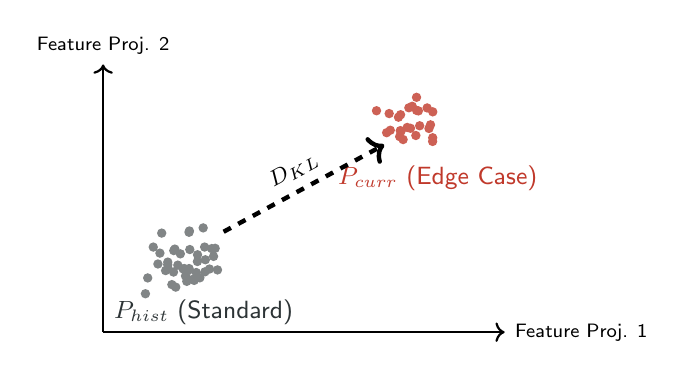
\begin{tikzpicture}[scale=0.85]
                % Axes
                \draw[->, thick] (0,0) -- (6,0) node[right] {\scriptsize Feature Proj. 1};
                \draw[->, thick] (0,0) -- (0,4) node[above] {\scriptsize Feature Proj. 2};
                
                % Hist Cloud (Blue Points)
                \foreach \x in {1, 1.2, 1.3, 1.5, 1.1, 1.4, 0.8}
                    \foreach \y in {1, 1.2, 0.9, 1.1, 1.3, 0.8}
                        \draw[fill=efblue!60, draw=none] (\x + rand*0.3, \y + rand*0.3) circle (2pt);
                
                \node[efblue] at (1.5, 0.3) {\small $P_{hist}$ (Standard)};
                
                % Curr Cloud (Red Points) - Shifted
                \foreach \x in {4.5, 4.7, 4.3, 4.8, 4.6}
                    \foreach \y in {3.0, 3.2, 2.8, 3.1, 3.3}
                        \draw[fill=efred!80, draw=none] (\x + rand*0.3, \y + rand*0.3) circle (2pt);
                        
                \node[efred] at (5.0, 2.3) {\small $P_{curr}$ (Edge Case)};
                
                % Shift Arrow
                \draw[->, ultra thick, dashed, black] (1.8, 1.5) -- (4.2, 2.8) 
                    node[midway, above, sloped] {\footnotesize \textbf{$D_{KL}$}};
                    
            \end{tikzpicture}
    \end{columns}
\end{frame}

\begin{frame}{Why RL? Intuition: Seeking Distributional Shifts}
    \textbf{Intuition:} We seek inputs that produce \textbf{large distributional shifts} ($D_{KL}$) relative to history. A large shift implies the batch hit a rare edge case or a novel internal state.
    
    \vspace{0.5cm}
    \centering
    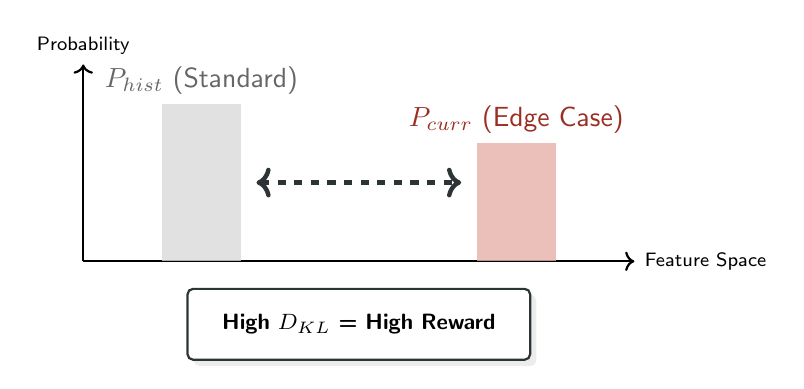
\begin{tikzpicture}[scale=1.0]
        % Axes
        \draw[->, thick] (0,0) -- (7,0) node[right] {\scriptsize Feature Space};
        \draw[->, thick] (0,0) -- (0,2.5) node[above] {\scriptsize Probability};
        
        % P_hist
        \fill[gray!30, opacity=0.8] (1,0) -- (1,2.0) -- (2,2.0) -- (2,0) -- cycle;
        \node[gray!80!black] at (1.5, 2.3) {$P_{hist}$ (Standard)};
        
        % P_curr
        \fill[efred!40, opacity=0.8] (5,0) -- (5,1.5) -- (6,1.5) -- (6,0) -- cycle;
        \node[efred!80!black] at (5.5, 1.8) {$P_{curr}$ (Edge Case)};
        
        % RL Connection - MOVED DOWN
        \draw[<->, ultra thick, efblue, dashed] (2.2, 1.0) -- (4.8, 1.0);
        \node[basicblock, fill=white, draw=efblue, text width=4cm] at (3.5, -0.8) {
            \textbf{High $D_{KL}$ = High Reward}\\
            % \scriptsize RL learns: This bucket reveals hidden boundaries!
        };
    \end{tikzpicture}
    
    \vspace{0.2cm}
    \centering
    \small \textbf{Role of RL:} To optimize the policy $\pi(s)$ to find buckets that maximize $D_{KL}$.
\end{frame}

% =================================================================
% 4. CASE STUDIES
% =================================================================
\section{Case Studies}

\begin{frame}{Case Study: Union Dirty Tail}
    \textbf{Context:} EIP-6800 \texttt{SuffixStateDiff}. Field \texttt{new\_value} is \texttt{Optional[Bytes32]} (Union).
    \textbf{Vulnerability:} \texttt{Selector=0x00} (None) should have 0 payload bytes.
    
    \vspace{0.5cm}
    \centering
    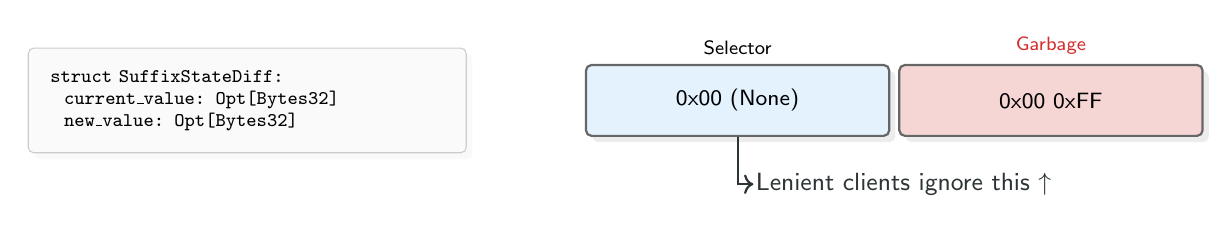
\begin{tikzpicture}[node distance=0cm]
        % Structure
        \node[codeblock, text width=5cm] (struct) {
            \textbf{struct SuffixStateDiff}:\\
            \ \ current\_value: Opt[Bytes32]\\
            \ \ new\_value: Opt[Bytes32]
        };

        % Selector
        \node[basicblock, right=1.5cm of struct, fill=fixedblue, label=above:\scriptsize Selector, minimum width=2.0cm] (sel) {0x00 (None)};
        
        % Garbage
        \node[basicblock, fill=alertred!20, right=0.1cm of sel, label=above:\scriptsize \textcolor{alertred}{Garbage}, minimum width=2.0cm] (tail) {0x00 0xFF};
        
        % Process
        \draw[->, thick, efblue] (sel.south) -- ++(0,-0.6) -- ++(0.2,0) 
            node[midway, right, font=\small] {Lenient clients ignore this $\uparrow$};
    \end{tikzpicture}
    
    \vspace{0.5cm}
    \begin{columns}[c]
        \column{0.5\textwidth}
        \textbf{Attack Scenario}
        \begin{itemize}
            \item \texttt{current\_value = None} (Selector 0x00).
            \item Attacker (proposer) appends trailing bytes.
        \end{itemize}

        \column{0.5\textwidth}
        \textbf{Impact}
        \begin{itemize}
            \item \textbf{Lenient client:} Decodes as None.
            \item \textbf{Strict client:} Rejects block.
            \item \textcolor{efred}{\textbf{Result: Consensus Split}}.
        \end{itemize}
    \end{columns}
\end{frame}

% =================================================================
% 5. RESULTS (DETAILED)
% =================================================================
\section{Evaluation}

\begin{frame}{Performance: TTE vs Baseline}
    \textbf{Data:} Median Time-To-Exposure over 30 runs.
    
    \vspace{0.2cm}
    Bug reproduction effectiveness on historical SSZ vulnerabilities. We report median TTE over 30 cold-start runs. ``--'' indicates the bug was not found within the 30-minute timeout.
    \vspace{0.2cm}
    
    \begin{table}
        \centering
        \small
        \resizebox{0.95\textwidth}{!}{%
        \renewcommand{\arraystretch}{1.3}
        \setlength{\tabcolsep}{10pt}
        \rowcolors{2}{white}{codebg}
        \begin{tabular}{lcccc}
            \toprule
            \textbf{Benchmark ID} & \textbf{Affected Implementations} & \textbf{Consensus Schema} & \textbf{LibFuzzer TTE (ms)} & \textbf{\tool{} TTE (ms)} \\
            \midrule
            BV-DirtyPadding & Prysm/fastssz, Teku, py-ssz & \icode{BeaconState.JustificationBits} & -- & \textbf{5.390} \\
            Bool-Dirty      & Prysm/fastssz, dynamic-ssz & \icode{Validator.Slashed} & -- & \textbf{0.351} \\
            Bitlist-Null    & dynamic-ssz & \icode{PendingAttestation.AggregationBits} & -- & \textbf{4.020} \\
            Union-DirtyTail & Lighthouse, Lodestar, remerkleable & \icode{SuffixStateDiff.new\_value} & -- & \textbf{0.164} \\
            Gap-Offsets     & remerkleable & \icode{PendingAttestation} & -- & \textbf{0.588} \\
            \bottomrule
        \end{tabular}
        }
    \end{table}
\end{frame}

\begin{frame}{Zero-Day Instances in Production Implementations}
    \small
    \textbf{Summary:} \tool{} uncovered \textbf{12} previously unknown vulnerability instances.
    
    \vspace{0.1cm}
    \textbf{Critical Impact (EIP-6800):} 
    The \textbf{Union} vulnerabilities (\#4.1--4.3) are \textbf{consensus-breaking}. EIP-6800 introduces \texttt{Optional[Bytes32]} (a Union) in the block header. Divergent handling of dirty tail bytes allows attackers to split the chain between strict and lenient clients.

    \vspace{0.2cm}
    \begin{table}
        \centering
        \scriptsize 
        \renewcommand{\arraystretch}{1.2}
        \setlength{\tabcolsep}{6pt}
        \rowcolors{2}{white}{codebg}
        \begin{tabular}{c l l}
            \toprule
            \textbf{\#} & \textbf{Vulnerability} & \textbf{Implementation / Issue} \\
            \midrule
            1 & Container short/empty input & Lodestar \href{https://github.com/ChainSafe/ssz/issues/502}{\texttt{ChainSafe/ssz\#502}} \\
            2.1 & Bitvector dirty padding & Teku \href{https://github.com/Consensys/teku/pull/10173}{\texttt{Consensys/teku\#10173}} \\
            2.2 & Bitvector dirty padding & Prysm (fastssz) \\
            2.3 & Bitvector dirty padding & ethereum/py-ssz \\
            2.4 & Bitvector dirty padding & dynamic-ssz \href{https://github.com/pk910/dynamic-ssz/issues/54}{\texttt{pk910/dynamic-ssz\#54}} \\
            3.1 & Boolean canon. \{0x00,0x01\} & fastssz \href{https://github.com/ferranbt/fastssz/issues/222}{\texttt{ferranbt/fastssz\#222}} \\
            3.2 & Boolean canon. \{0x00,0x01\} & dynamic-ssz \href{https://github.com/pk910/dynamic-ssz/issues/53}{\texttt{pk910/dynamic-ssz\#53}} \\
            \hline
            \rowcolor{efred!15} 4.1 & Union trailing data & Lighthouse \href{https://github.com/sigp/ethereum_ssz/issues/64}{\texttt{sigp/ethereum\_ssz\#64}} \\
            \rowcolor{efred!15} 4.2 & Union trailing data & Lodestar \href{https://github.com/ChainSafe/ssz/issues/507}{\texttt{ChainSafe/ssz\#507}} \\
            \rowcolor{efred!15} 4.3 & Union trailing data & remerkleable \href{https://github.com/protolambda/remerkleable/issues/28}{\texttt{protolambda/remerkleable\#28}} \\
            \hline
            5 & Container gap & remerkleable \href{https://github.com/protolambda/remerkleable/issues/29}{\texttt{protolambda/remerkleable\#29}} \\
            6 & Null-bitlist trap & dynamic-ssz \href{https://github.com/pk910/dynamic-ssz/issues/56}{\texttt{pk910/dynamic-ssz\#56}} \\
            \bottomrule
        \end{tabular}
    \end{table}
\end{frame}


% =================================================================
% 6. CONCLUSION
% =================================================================
\section{Conclusion}

\begin{frame}{Summary} 
    \begin{columns}[c]
        \column{0.6\textwidth}
        \textbf{Summary}
        \begin{itemize}
            \setlength\itemsep{0.5em}
            \item \textbf{Risk:} SSZ logic bugs cause silent consensus splits.
            \item \textbf{Solution:} Spec-Guided Abstraction + RL.
            \item \textbf{Impact:} Found 12 Zero-days in 4 industry-leading Ethereum consensus clients (10k+ GitHub stars, powering 80\% of Ethereum validators). 
        \end{itemize}
        
        % \vspace{0.5cm}
        % \textbf{Next Steps}
        % \begin{itemize}
        %     \setlength\itemsep{0.5em}
        %     \item Add ``Refusal Vectors'' to \texttt{consensus-specs}.
        %     \item Integrate \tool into Client CI pipelines.
        % \end{itemize}

        \column{0.4\textwidth}
        \centering
        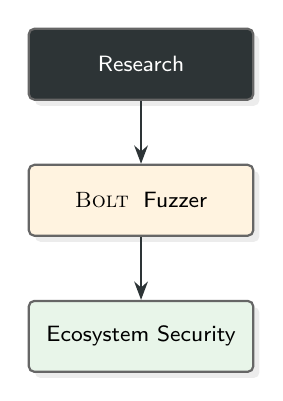
\begin{tikzpicture}[node distance=0.8cm]
            \node[basicblock, fill=efblue, text=white, text width=2.5cm] (res) {Research};
            \node[basicblock, below=of res, fill=offsetorange, text width=2.5cm] (tool) {\tool \; Fuzzer};
            \node[basicblock, below=of tool, fill=heapgreen, text width=2.5cm] (eco) {Ecosystem Security};
            
            \draw[flow] (res) -- (tool);
            \draw[flow] (tool) -- (eco);
        \end{tikzpicture}
    \end{columns}
\end{frame}


\begin{frame}{The Big Picture: Ethereum Consensus Architecture}
    \textbf{Current Status:} We have successfully secured the \textbf{Serialization Layer}.
    Deep logic bugs inside the state machine remain a challenge for future work.
    
    \vspace{0.4cm}
    \centering
    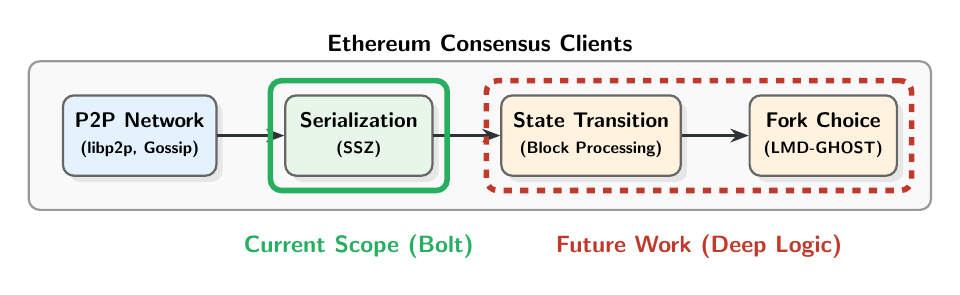
\begin{tikzpicture}[node distance=1.2cm, auto, scale=0.85, transform shape]
        % Horizontal Flow
        \node[moduleblock, fill=fixedblue] (p2p) {P2P Network\\ \scriptsize (libp2p, Gossip)};
        \node[moduleblock, fill=heapgreen, right=1.0cm of p2p] (ssz) {Serialization\\ \scriptsize (SSZ)};
        \node[moduleblock, fill=offsetorange, right=1.0cm of ssz] (stf) {State Transition\\ \scriptsize (Block Processing)};
        \node[moduleblock, fill=offsetorange, right=1.0cm of stf] (fc) {Fork Choice\\ \scriptsize (LMD-GHOST)};
        
        % Background Box
        \begin{scope}[on background layer]
            \node[draw=black!40, fill=gray!5, thick, rounded corners=4pt, fit=(p2p)(fc), inner sep=12pt, label={[font=\bfseries]north:Ethereum Consensus Clients}] (client) {};
        \end{scope}

        % Arrows
        \draw[flow] (p2p) -- (ssz);
        \draw[flow] (ssz) -- (stf);
        \draw[flow] (stf) -- (fc);
        
        % Scopes - Adjusted labels to stay inside/aligned
        \node[draw=efgreen, line width=2pt, rounded corners, fit=(ssz), inner sep=5pt, label={[text=efgreen, font=\bfseries, yshift=-0.5cm]below:Current Scope (\tool)}] {};
        
        \node[draw=efred, dashed, line width=2pt, rounded corners, fit=(stf)(fc), inner sep=5pt, label={[text=efred, font=\bfseries, yshift=-0.5cm]below:Future Work (Deep Logic)}] {};
        
    \end{tikzpicture}
\end{frame}

\begin{frame}{Future Direction: Fuzzing for State Transition \& Fork Choice}
    \textbf{Extending the Technique:} Apply Distributional RL + Differential Fuzzing to deep consensus logic.
    
    \vspace{0.5cm}
    \centering
    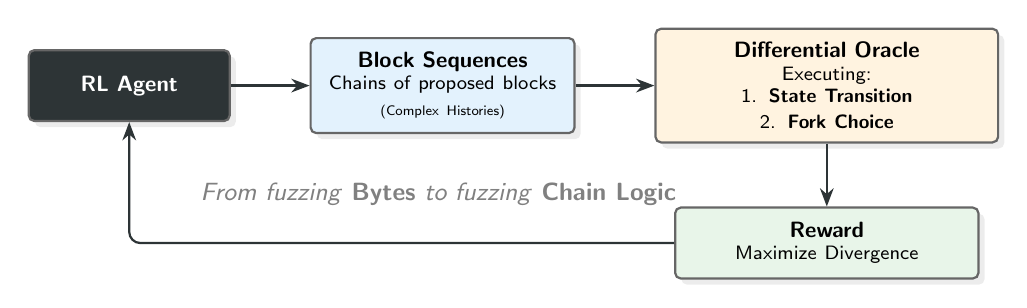
\begin{tikzpicture}[node distance=1.2cm, auto]
        % Agent
        \node[basicblock, fill=efblue, text=white, text width=2.2cm] (agent) {\textbf{RL Agent}};
        
        % Input
        \node[basicblock, right=1.0cm of agent, fill=fixedblue, text width=3.0cm] (input) {
            \textbf{Block Sequences}\\
            \scriptsize Chains of proposed blocks\\
            \tiny (Complex Histories)
        };
        
        % Oracle
        \node[basicblock, right=1.0cm of input, fill=offsetorange, text width=4.0cm] (oracle) {
            \textbf{Differential Oracle}\\
            \scriptsize Executing:\\
            \scriptsize 1. \textbf{State Transition}\\
            \scriptsize 2. \textbf{Fork Choice}
        };
        
        % Reward
        \node[basicblock, below=0.8cm of oracle, fill=heapgreen, text width=3.5cm] (reward) {
            \textbf{Reward}\\
            \scriptsize Maximize Divergence\\
        };
        
        % Loops
        \draw[flow] (agent) -- (input);
        \draw[flow] (input) -- (oracle);
        \draw[flow] (oracle) -- (reward);
        \draw[flow] (reward) -| (agent);
        
        % Insight
        \node[below=0.5cm of input, font=\small, color=gray, align=center] {
            \textit{From fuzzing \textbf{Bytes} to fuzzing \textbf{Chain Logic}}
        };
        
    \end{tikzpicture}
\end{frame}

% \begin{frame}
%     \centering
%     \Huge \textbf{Questions?}
    
%     \vspace{1cm}
%     \normalsize
%     \textbf{Artifacts Available:}\\
%     \texttt{https://github.com/.../bolt}
% \end{frame}

\end{document}